\chapter{Soluções existentes e objetivos}
\label{c.solucoes-existentes-e-objetivos}

% https://capozzielli.gdigital.com.br/usuario/

% https://www.techtudo.com.br/tudo-sobre/bo-coletivo.html
% No Brasil, o aplicativo \emph{BO coletivo} permite com que os usuários colaborem com um mapeamento coletivo de assaltos, furtos, roubos e sequestros. Porém, ele é útil apenas para consultas posteriores, não oferecendo mecanismos para ações preventivadas em tempo real, e também, em relação à usabilidade, o aplicativo não permite a navegação pelo mapa ao digitar uma região desejada.

Ao analisar as diferentes soluções que já resolvem o problema destacado, é possível definir qual o objetivo da solução desenvolvida neste trabalho.

\section{Soluções existentes}

Já existem soluções para o mesmo problema tanto no Brasil como no mundo, porém elas possuem diferentes abordagens.

% - Deve-se fazer uma pesquisa de soluções existentes para o mesmo problema que deseja resolver.
% - As soluções pesquisadas devem ser descritas com profundidade suficiente para que fique caracterizada sua competência em resolver o problema em questão, bem como seus aspectos positivos e negativos.

\subsection{Citizen}

O aplicativo \emph{Citizen} ~\cite{citizen}, desenvolvido pela \emph{sp0n, Inc.}, foi lançado originalmente em 2016 com o nome de \emph{Vigilante} em alguns grandes centros dos Estados Unidos. Em junho de 2020, ele possuía cerca de 5 milhões de usuários ativos. Seu sucesso vem da sua robustez, usabilidade, velocidade e praticidade. Entre as principais funcionalidades destacam-se o envio de alertas de segurança baseado na localização em tempo real, o acompanhamento pelos usuários dos alertas que estão em andamento, a transmissão de vídeos ao vivo e a possibilidade de adicionar comentários. As suas notificações já ajudaram pessoas à evacuarem de prédios em chamas e ônibus escolares à escaparem de ataques terroristas. 

A empresa dona do aplicativo, \emph{sp0n, Inc}, possui antenas de rádio nas cidades suportadas para que as chamadas telefônicas da polícia local sejam monitadoras, permitindo com que operadores especializados da empresa as filtrem e publiquem alertas no aplicativo. Em razão disso, o aplicativo \emph{Citizen} tem sua atuação dependente dos orgãos públicos. Em agosto de 2020, ele atuava em apenas 60 cidades dos Estados Unidos.

A Figura~\ref{f.citizen} mostra algumas das principais telas do aplicativo.

\begin{figure}[htbp]
	\caption{\small Telas do aplicativo Citizen.}
	\centering
	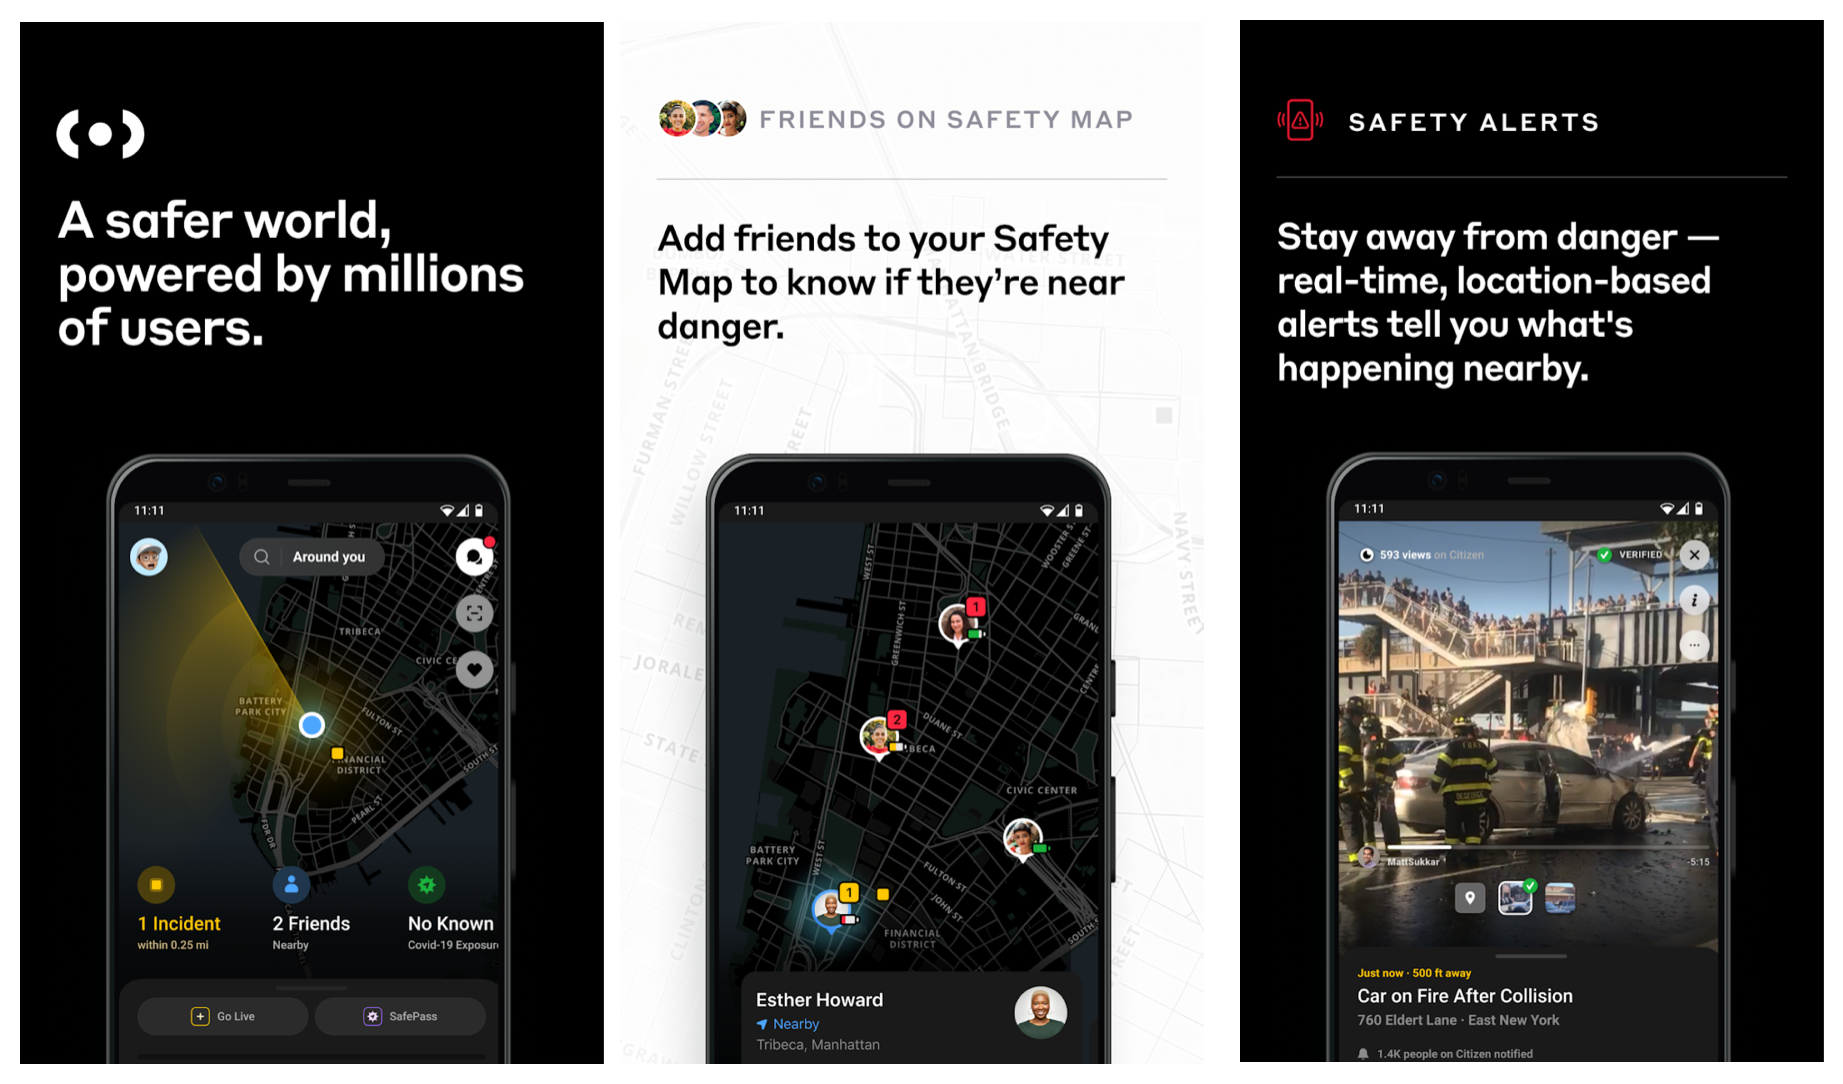
\includegraphics[height=8cm]{./images/citizen.png}
	\label{f.citizen}
	\legend{\small Fonte: Google Play, 2022.}
\end{figure}

\FloatBarrier

\subsection{SP+ segura}

O aplicativo \emph{SP+ segura} ~\cite{sp-mais-segura} foi lançado pela Secretaria Municipal de Segurança Urbana de São Paulo em novembro de 2017. Com mais de 50 mil usuários, o aplicativo permite com que pessoas informem e sejam informadas de alertas em tempo real sobre episódios de risco em que pessoas se encontram ou presenciam. 

Ele oferece a opção de ligar para o orgão público responsável para acioná-lo quando for necessário. Porém, ele não oferece interação de chat entre usuários para eventuais discussões, e não suporta o envio de vídeos. Além disso, conta com muitas avaliações negativas na loja de aplicativos pelos usuários, com criticas à baixa qualidade. A Figura~\ref{f.sp-mais-segura} mostra as principais telas do aplicativo.

\begin{figure}[htbp]
	\caption{\small Telas do aplicativo SP+ segura.}
	\centering
	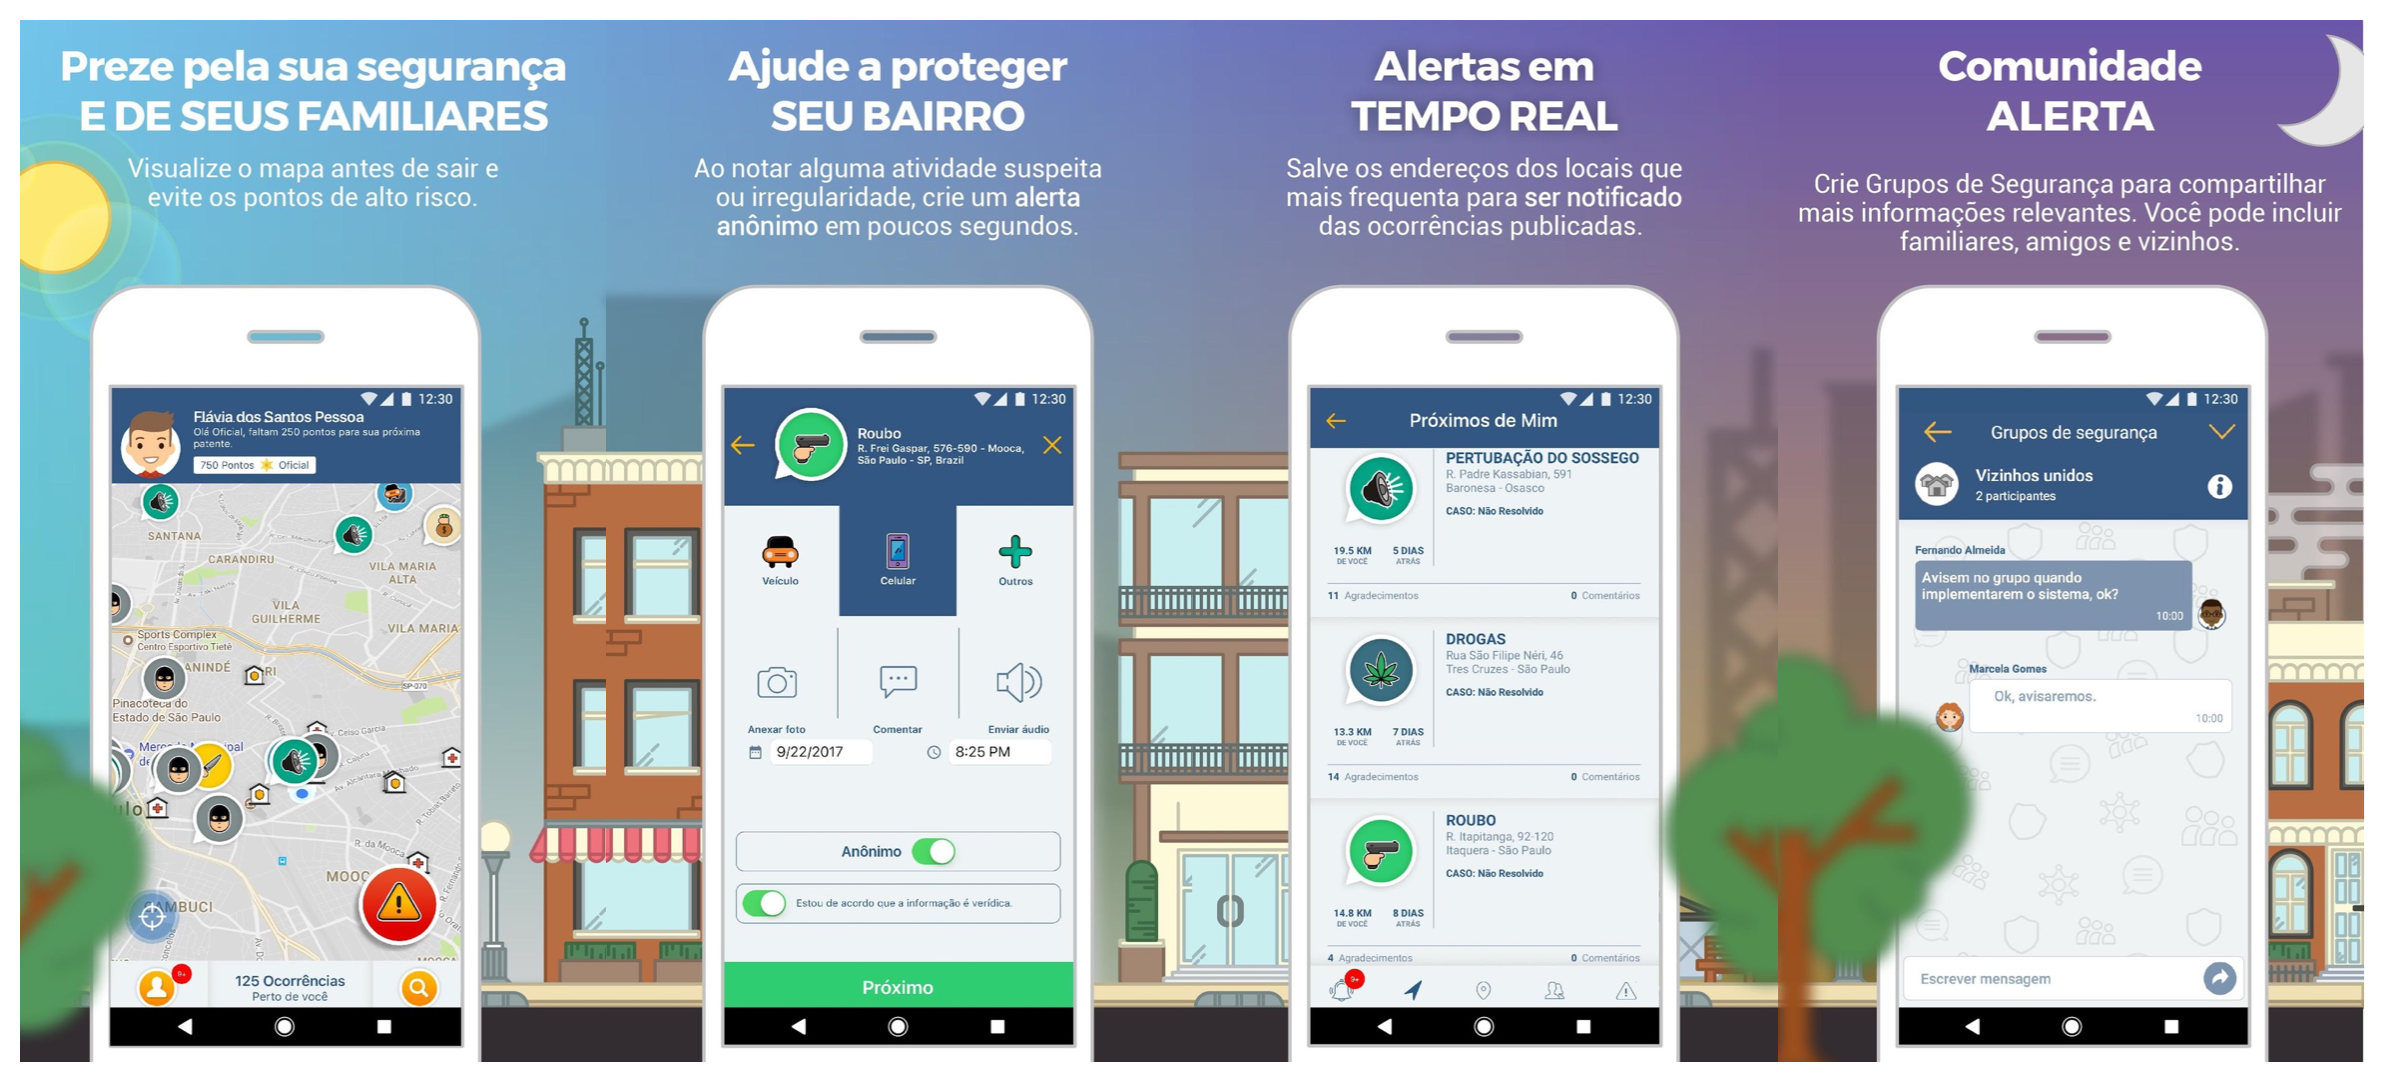
\includegraphics[width=\textwidth]{./images/sp-mais-segura.png}
	\label{f.sp-mais-segura}
	\legend{\small Fonte: Google Play, 2022.}
\end{figure}

\FloatBarrier

\subsection{Análise}
% - Ao final da seção deverá ser feita uma análise crítica das soluções existentes.
% - Como base nessa análise, os objetivos do projeto proposto deverão ser descritos de forma a caracterizar claramente suas diferenças em relação aos projetos existentes.

Dada as soluções existentes descritas, nota-se que o \emph{Citizen} é a maior referência do segmento no mundo. Porém, apesar de seu enorme sucesso, ele é restrito à apenas algumas cidades dos Estados Unidos e não apresenta previsão de expansão para o Brasil. O Brasil possui soluções para o problema, porém elas não apresentam a mesma qualidade. Portanto, surgiu-se a oportunidade de oferecer uma solução alternativa.

\section{Objetivos}

% Esta especificação tem por objetivo definir em detalhes o trabalho que será desenvolvido na disciplina de TCC. Nessa fase, o aluno deve cumprir quatro objetivos fundamentais:

% a) Descrever claramente o problema que deseja resolver e sua motivação.  
% b) Pesquisar soluções existentes para o problema que deseja resolver.
% c) Propor uma solução alternativa para o problema, caracterizando as diferenças com as soluções existentes.
% d) Pesquisar as tecnologias e ferramentas que poderão ser utilizadas em seu projeto, a fim de avaliar sua viabilidade.

Este trabalho tem como objetivo apresentar o processo e as atividades para o desenvolvimento de uma aplicação móvel onde as pessoas possam se manter conscientes, em tempo real, de situações de perigo que eventualmente podem estar ocorrendo nas suas proximidades, como crimes, incêndios, ameaças, protestos, ruas interditadas, catástrofes naturais, entre outros. O aplicativo deve oferecer a infraestrutura para o desenvolvimento de um senso de comunidade. A integração dos alertas com os chamados das polícias locais não está incluso no escopo do projeto.
